\subsection{Mars}

\initial{F}irst, we look at Mars. 
Mars is by far the most explored planet besides Earth. 
How are we going to continue the exploration in the future?
President Barack Obama has tasked NASA with the goal of getting astronauts to Mars, or in Mars' orbit by the mid-2030s. 
This, as well as the Mars One-program, aiming to establish a permanent human settlement on Mars \cite{FPlan12}, has shaped the exploration strategy. 
So far, the only question has been \emph{"are we alone?"} 
The new strategy poses another, more critical question; \emph{"is it safe for humans?"} \cite{FPlan01}.

\subsubsection{Mars 2020 rover}

The Mars 2020 rover mission is NASAs next contribution to the exploration of the red planet. 
Building on Curiositys great landing system, the mission will launch in 2020 taking advantage of the favorable orbital positions of Mars and Earth \cite{FPlan14}. 

\begin{center}
	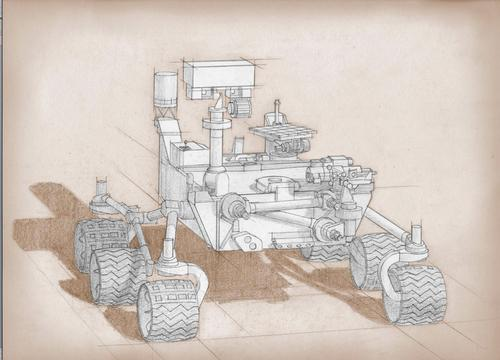
\includegraphics[width=0.45\textwidth]{2020_Rover_Sketch.jpg}
\end{center}
The 2020 mission has four main goals \cite{FPlan13}.

\begin{enumerate}
	\item \textbf{Determine whether life ever existed on Mars}
The rover is going to look for signs of biosignatures preserved in rock samples formed in the ancient Martian environment.
This will be the first rover to seek for actual signs of past microbial life.
	\item \textbf{Characterize the Climate of Mars}
The rover will look for signs that Mars might have provided a habitable environment for microbial life in the past. 
	\item \textbf{Characterize the Geology of Mars}
Studying the processes that created and modified the Martian surface by examining the rock record.
Every layer of rock in the Martian crust reveals a record of the environment in which it was formed.
	\item \textbf{Prepare for Human Exploration}
This goal relates to the American national space policy of getting an astronaut to Mars by the mid-2030s.
The rover will demonstrate key technologies for using natural resources in the Martian environment for fuel and life support. 
\end{enumerate}

It will also measure environmental conditions that might be hazardous for future human travellers.

\end{multicols}

{%kilde: http://www.telegraph.co.uk/news/science/space/10200818/Dangers-of-a-manned-mission-to-Mars.html

\begin{tcolorbox}[colback=green!5,colframe=green!40!black,title=5 dangers for humans to overcome at Mars]
\textbf{Atmosphere:} It is impossible to breath in, due to its low density, as well as its high complex of carbon dioxide.

\textbf{Radiation:} There is constant background radiation on Mars, but there is also a much stronger direct radiation from the Sun. With no significant protection from the Martian atmosphere or a planet wide magnetic field, radiation can reach intensities enough to ionise atoms and thus split chemical compounds, making the environment though to any living creature we know of.

\textbf{Climate:} Liquid water is not known to occur on Mars, however the poles have permafrost. The warmest climate, and thus the most friendly to humans, on Mars is to be found around its equator.

\textbf{Meteorites:} Mars is located near an asteroid belt, and with weak protection from the atmosphere, the Martian surface gives a clue on how great consequences these impacts may cause.

\textbf{Health:} Living in low gravity causes the human body to slowly fall apart. This is crucial when travelling to Mars, but could also be significant at the Martian surface. It is also expected that isolation so far from home could affect the traveller's mental health.
\end{tcolorbox}}

\begin{multicols}{2}

\subsubsection{ExoMars}

ESA (the European Space Agency) considers the question 'did life ever exist on Mars?' as one of the most important scientific questions of our time.
To address this the ExoMars-program was established.
The goal of the mission is to investigate the Martian environment and to demonstrate new technologies paving way for a future Mars sample return mission in the 2020’s \cite{FPlan02}. 
The ExoMars-program are divided into two missions.
The first consisting of an orbiter (Trace Gas Orbiter) plus an entry, descent and landing demonstrator module (launches in January 2016).
The second featuring a rover dated to launch in 2018.
 
\begin{center}
	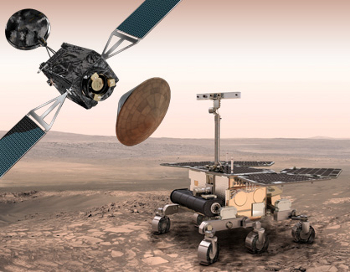
\includegraphics[width=0.45\textwidth]{ExoMars.jpg}
\end{center}

The ExoMars Trace Gas Orbiters main objective is to search for evidence of gases of possible biological importance in the Martian atmosphere, such as methane and its degradation products.
It will also serve as a data relay asset for the 2018 rover mission.
The ExoMars Entry, Descent and Landing Demonstrator Module’s (EDM) objective is to provide ESA with the necessary technology for a controlled landing on the surface of Mars.
The EDM is not going to survive on Mars.
After a short time the batteries runs out and the module shuts down.
Scientific recordings are limited; however, some sensors will be included to preform limited, but useful measurements.
After a nine-month journey, the ExoMars rover hopefully lands unharmed on the surface of Mars.
The rover’s main objective is to travel across the Martian terrain and search for signs of life.
ExoMars will be the first mission to combine the ability to move across the surface and to examine Mars at depth.
With a drill capable of reaching a depth of two meters, it collects samples and analyze them with next-generation instruments.
The goal is to identify organic material from the planets early history.

\subsubsection{Sample return mission}

A sample return mission (MSR) would collect a sample of ruck and dust on the surface of Mars to return to Earth.
This would be a giant leap in the exploration of Mars because it frees us from the time, budged and space constraints of spacecraft sensors.
All of Earth’s laboratories could potentially study the samples \cite{EarthAnalysis}.
 
\begin{center}
	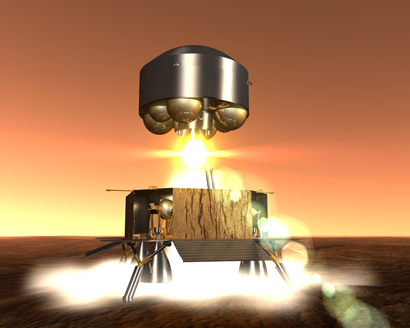
\includegraphics[width=0.45\textwidth]{Sample_return_concept.jpg}
\end{center}

Initially the ExoMars program was a joint project between NASA and ESA with the final goal of a sample return in the mid-2020s \cite{FPlan15}.
Under the FY2013 budget President Barack Obama released in early February 2012, NASA had to withdraw from the joint missions because of budget cuts \cite{FPlan16}.
ESA continues the program without NASA, but there is still no fixed launch date for a sample return mission.
Russia and China are also working on concepts for a sample return mission without any specific timeframes \cite{RussiaPlan} \cite{ChinaPlan}.

\initial{M}ars is by far the most investigated planet besides from Earth.
There have been spent enormous amounts of money on the search for water and signs of biosignatures, but is Mars the best choice to search for life?
Are there other candidates suitable for supporting life? 
As mentioned on numerous occasions, liquid water is a key factor when we are talking about life. 
The Goldilocks zone describes the region in space where a planet has just the right distance from its home star resulting in neither too hot nor too cold temperatures for liquid water to exist \cite{FPlan26}. 
Our solar system turns out to be quite an interesting place, where liquid water is found on numerous unexpected locations. 
Dr. McKay, who studies the possibility of life in alien worlds, states: \emph{"after spending so many years going after Mars, which is so dry and so bereft of organics and so just plain dead, it is wonderful to go to the outer solar system and find water, water everywhere!"} \cite{FPlan09}.
Where is this water we are talking about, and how are we going to search for life there?


\subsection{Europa}

\begin{tcolorbox}[colback=red!5,colframe=DarkRed!40!black,title=Europa \cite{Europa}]

{\centering
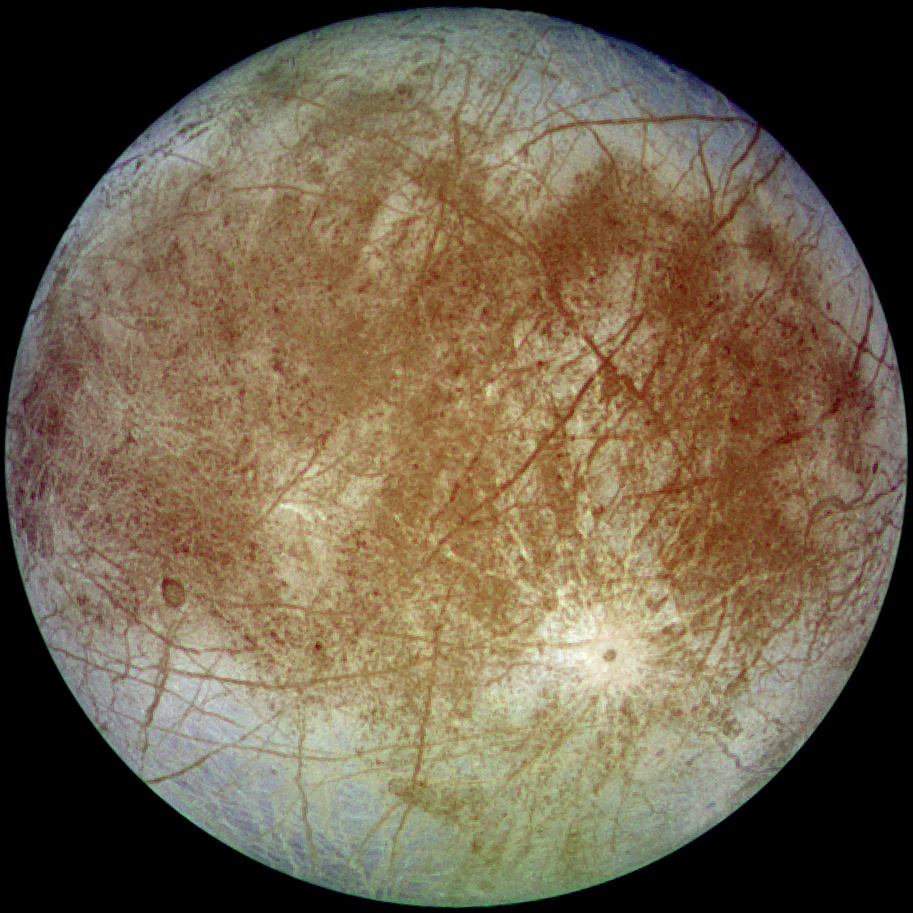
\includegraphics[width=\textwidth]{Europa_moon.jpg}
\par}

\textbf{Satellite of:} Jupiter

\textbf{Diameter:} $3120km$ ($0.245$ Earths)

\textbf{Mass:} $4.8\cdot 10^{22}kg$ ($0.008$ Earths)

\textbf{Surface temp.:} $-171.15\degree C$

\textbf{Gravity:} $0.13 G$s

\textbf{Surface pressure:} $10^{-12} atm.$
\end{tcolorbox}

% solarsytem.nasa.gov/planets/profile.cmf?Object=Jup_Europa&Display=Facts
% Name Europa: Facts & Figures
% Date 22.04.15
 
\initial{E}uropa is one of Jupiter's 64 moons.
With a diameter of 3121.6 km, it is the sixth largest moon in the solar system and would be classified as a dwarf-planet (just like Pluto) if it orbited the sun.
With a mean surface temperature of -171.15\degree C, this is indeed a very cold world.
Ice covers the entire surface, and the atmosphere is weary thin, about 10-12 times earth's atmosphere.
At first glance, it does not look habitable, but scientists actually believe this to be one of the most likely places to find life in our solar system.
Because of tidal flexing, a process caused by Jupiter’s strong gravity and Europa’s slightly eccentric orbit as well as orbital resonance with the other moons, it generates heat melting the ice from inside.
Scientists believe the moon to have a 100 km thick layer of liquid water under 30 km of ice \cite{FPlan03} \cite{FPlan24}.
 
In 1977, scientists discovered life independent of sunlight concentrated around underwater volcanic features known as black smokers.
In addition, it was recently discovered bacterial life in a Lake Whillans 800 meters below the Antarctic icecap \cite{FPlan04}. This strengthen the theory of life on Europa.
There are currently three different projects in work to look for life on Europa: Juice, Europa Clipper and Valkyrie \cite{FPlan24}.
Juice is an ESA engaged mission featuring an orbiter planned to launch in 2022.
The orbiter is going to visit the Jupiter moons Europa, Callisto and Ganymedes.
It is only going to pass Europa twice in which time it will measure the thickness of the ice as well as mapping the surface in detail.
The wide range of instruments will also reveal the moons internal structure and chemical environment \cite{FPlan24}.
NASA is also going to send an orbiter planned to launch in 2025.
The spacecraft is going to pass Europa 45 times while orbiting Jupiter.
With a variety of instruments shall examine the same factors that Juice \cite{FPlan24}.
Most exiting is the NASA engaged mission Valkyrie.
Valkyrie is an autonomous robot that will drill through the thick ice and explore the ocean underneath it.
The robot consists of a long cigar formed tube melting its way through the ice powered by a 5000-watt laser carried through a fibre optic wire from a nuclear power source on the surface.
Tests conducted in Alaska have shown that Valkyrie is able to move at a rate of almost one meter per hour \cite{FPlan24} \cite{FPlan25}.

\subsection{Titan}

\begin{tcolorbox}[colback=red!5,colframe=DarkRed!40!black,title=Titan \cite{Titan}]

{\centering
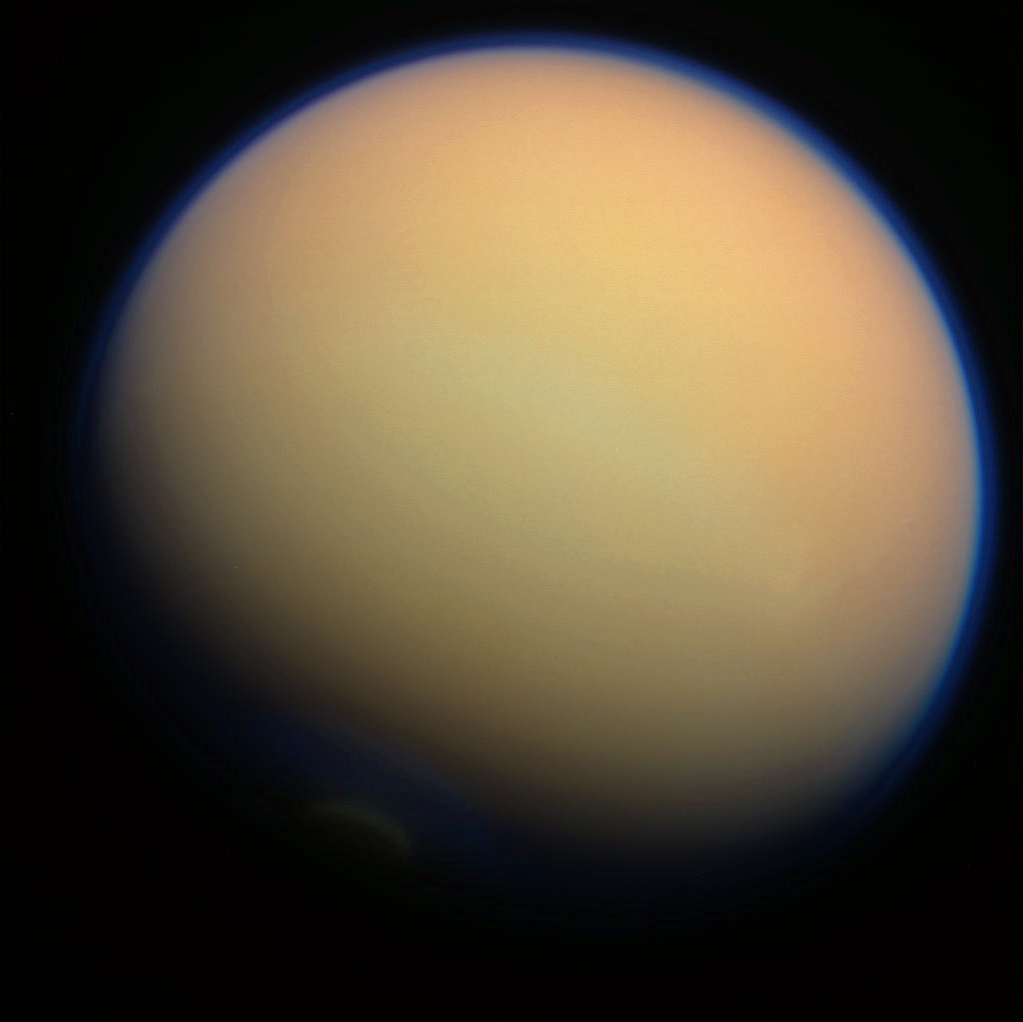
\includegraphics[width=\textwidth]{Titan_moon.jpg}
\par}

\textbf{Satellite of:} Saturn

\textbf{Mean diameter:} $5,150km$ ($0.404$ Earths)

\textbf{Mass:} $1.35\cdot 10^{23}kg$ ($0.023$ Earths)

\textbf{Surface temp.:} $-179.5\degree C$

\textbf{Gravity:} $0.14 G$s

\textbf{Surface pressure:} $1.45 atm.$
\end{tcolorbox}

% http://solarsystem.nasa.gov/planets/profile.cfm?Object=Sat_Titan&Display=Facts
% Name Titan: Facts & Figures
% Date 22.04.15
 
\initial{T}itan, one of Saturn's 62 moons, have also caught scientists' attention.
With a diameter of 5150 km, it is the second largest moon in the solar system, and just like Europa, Titan is very cold.
Receiving only 1\% of sunlight compared to earth the surface temperature is about -180\degree C.
Titan is actually the only known moon with a significant atmosphere, and despite the lower gravity, it has a larger atmospheric pressure than earth (about 1.45 atm.).
What intrigues scientists is the environmental similarities with the theoretical primordial Earth.
Titan is thought to be a prebiotic environment rich on complex organic chemistry \cite{RichOrganics}. On the other hand, the lack of liquid water have led some scientists to consider life as unlikely.
However, Titan is rich on other compounds like for hydrocarbons a.m.
These could replace water as a solvent (read more about this hypothesis later).
Resent years it is proposed several interesting conceptual missions for sending a space probe to Titan. Unfortunately, all of these have yet to be funded.
The Titan Saturn System Mission (TSSM) was created by merging ESA’s Titan and Enceladus Mission (TandEM) with NASA’s Titan Explorer in January 2009 \cite{FPlan10}.
TSSM was an ambitious mission featuring a hot air balloon flying in Titans thick atmosphere.
Carried by the winds it could circle the moon in only six months and would have managed two circumnavigation in its design one-year lifetime.
Early February 2009 ESA and NASA announced that a Europa-Jupiter mission had priority ahead of TSSM \cite{FPlan07}.
It has also been proposed two different concepts featuring a lake-lander, TiME (Titan Mare Explorer) and TALISE (Titian Lake In-situ Sampling Propelled Explorer).
Splashing into a lake on the northern hemisphere, it would float in the cold methane liquids \cite{TiME} \cite{TALISE}.
In addition, a mission consisting of an unmanned drone (AVIATR) was proposed in early 2012, but NASA did not approve the requested \$ 715 million for the project \cite{AVIATR}.

\subsection{Enceladus}

\begin{tcolorbox}[colback=red!5,colframe=DarkRed!40!black,title=Enceladus]

{\centering
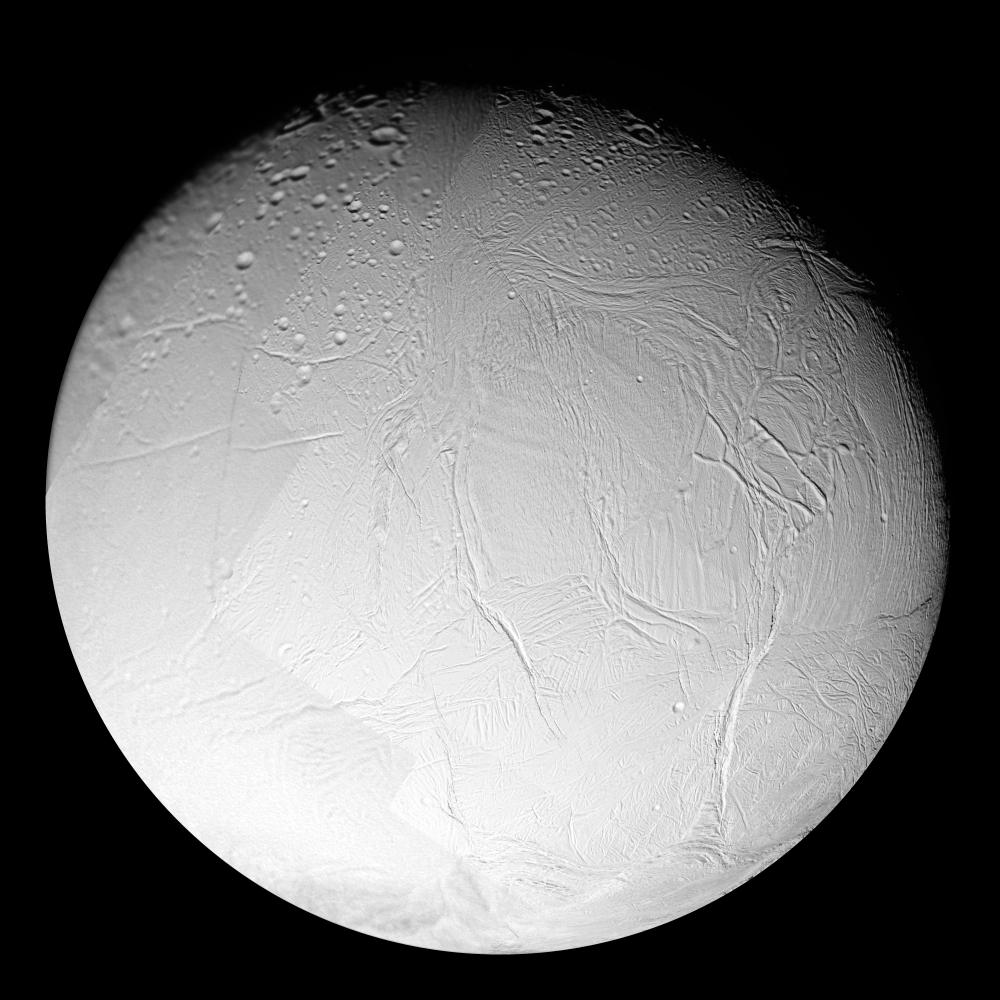
\includegraphics[width=\textwidth]{Enceladus_moon.jpg}
\par}

\textbf{Satellite of:} Saturn

\textbf{Mean diametre:} &504km& (&0.04& Earths)

\textbf{Mass:} $1.08 \cdot 10^{20}kg$ (&1.8 \cdot 10^{-5}& Earths)

\textbf{Surface temp.:} &-178 \degree C&

\textbf{Gravity:} &0.012 G&s

\textbf{Surface pressure:} &---&
\end{tcolorbox}

% solarsystem.nasa.gov/planets/profile.cmf?Object=Sat_Enceladus&Display=Facts
% Enceladus: Facts & Figures
% Date 22.04.15
 
\initial{E}nceladus, another of Saturn’s 62 moons turns out to be more interesting than previously assumed.
With a radius of only 500 km, it is much smaller than Titan, but still the sixth largest orbiting Saturn.
Just like Europa and Titan, Enceladus is very cold.
With a mean temperature at approximately -198\degree C, ice covers the entire surface.
Before the Cassini spacecraft started multiple close flybys in 2005 Enceladus was thought to have liquid water under the ice.
When the flybys started, it discovered cryovolcanoes near the South Pole shooting geyser-like jets with velocities up to 2189 km/h (equivalent to 1.8 times Mach 1 under normal conditions on Earth) into space.
Measurements revealed that the cryovolcanoes consisted of water vapor, other volatiles, and solid material like crystals and ice particles \cite{Enceladus1}.
Scientists’ also reports evidence of hydrothermal vents.
If this turns out to be correct, Enceladus would be the only known place, besides from earth, with such chemical reactions between rock and heated water \cite{FPlan09}.
The Cassini missions have provided evidence of several nutrients and organic molecules.
The combination of an internal salty ocean with hydrothermal vents and simple organic compounds makes this a potentially habitable environment for microbial extraterrestrial life.
The Titan and Enceladus Mission (TandEM) was, before merging with NASAs Titan Explorer (crating Titan Saturn System Mission, TSSM), a mission to study the Saturnian moons Titan and Enceladus, with special emphasis on Enceladus \cite{FPlan11}.
TSSM mainly focused on Titan but the missions’ orbiter would do a minimum of seven close flybys analyzing the cryovolcanic plumes.
There are unfortunately no current plans to send a spacecraft to Enceladus, or Titan for that matter.
Both NASA and ESA seems to focus on Europa first.

\subsection{Other possible goals}

\initial{B}oth Ganymede and Callisto (moons of Jupiter) seems to have hidden water under the surface \cite{FPlan09}.
Every place in the universe harboring liquid water is considered interesting and the moons could potentially support life, though less likely than Europa, Titan and Enceladus.
Scientists has also pointed out Venus as a potential place to habitat life.
At first glance, it might not look habitable.
With a mean surface temperature of 462\degree C (hot enough to melt led) and an atmospheric pressure 90 times that on Earth even the spacecraft that landed on Venus was crushed and melted within a couple of hours \cite{FPlan17} \cite{FPlan18}.
However, reputable scientists like Carl Sagan, David Grinspoon, Geoffrey A. Landis and Dirk Schulze-Makuch suggest a hypothesis of microbes existing in cloud layers 50 km above the surface \cite{LifeVenus}.
Temperatures here would be refreshingly tolerable.
Atmospheric sulfur dioxide and carbon monoxide might serve as food for the floating microbes \cite{FPlan20}.

Ceres is the largest known object in the asteroid belt, but still the smallest known dwarf planet \cite{FPlan21}.
On March 6, 2013, infrared readings from the Herschel space observatory confirmed water vapor rising from the surface. It is suggested that Ceres possess subsurface liquid water, and perhaps traces of life \cite{FPlan22}.
The Dawn mission, led by NASA, is the only spacecraft that has visited Ceres \cite{FPlan23}.
It has neither confirmed nor disproved the theory of liquid water.
